% File: main.tex
% Author: Auto-Intern GmbH
% Manuals template
\newcommand{\fach}{Digitaltechnikpraktikum }
\newcommand{\titelname}{Versuchsprotokoll }
\newcommand{\matrikel}{2016507006 }
\newcommand{\name}{Olbrich, Marie }

\newcommand{\matrikelpartner}{2016506999 }
\newcommand{\namepartner}{Hoffmann, Manuel }

\newcommand{\versuchsbezeichnung}{DT4 }
\newcommand{\versuchsname}{Entwurf eines BCD -> 7-Segment-Kodeumsetzers und Realisierung mittels eines CPLD Bausteines }
\newcommand{\semester}{SS17 }
\newcommand{\datum}{25.04.2017 }
\newcommand{\betreuer}{M.Sc. Kruse }
\newcommand{\dozent}{M.Sc. Richthofer }

\documentclass[a4paper, 11pt, fleqn, DIV=10, twoside, BCOR=10mm]{scrreprt}
\usepackage{diagbox}

%%%% Eingebundene Pakete %%%% 
\usepackage{xltxtra}

\usepackage{scrhack} 
\usepackage{xcolor}
\usepackage{color}
\usepackage{xfrac} % \sfrac{}{} für Brueche
\usepackage{graphicx}
\usepackage{float}
\usepackage{subcaption}
\usepackage{setspace}
\usepackage{wrapfig}
\usepackage{longtable}
\usepackage{geometry}
\usepackage{scrlayer-scrpage}
\usepackage{wallpaper}
\usepackage{ulem}
\usepackage{siunitx}
\usepackage{amsmath}
\usepackage{chngcntr}

%% Sorgt dafür, dass Kapitel neue Kapitel nicht auf einer neuen rechten Seite anfangen
\RedeclareSectionCommand[style=section,indent=0pt]{chapter}

%% Definition der Auto Intern Farben (Das AIschwarz wir im Fließtext nicht benutzt, stattdessen ist normales schwarz gesetzt (schwarze Tinte beim Druck günstiger)
\definecolor{THrot}{RGB}{228,0,30}
\definecolor{THblau}{RGB}{0,61,125}



%% Auto-Intern vereinfachte Befehle für Schriftarten
\newcommand{\mainfont}{\setmainfont{Lato-Regular.ttf}}
\newcommand{\LatoReg}{\setmainfont{Lato-Regular.ttf}}
\newcommand{\DaysOne}{\setmainfont{DaysOne-Regular.ttf}}
\newcommand{\LatoBold}{\setmainfont{Lato-Bold.ttf}}
\newcommand{\Avenir}{\setmainfont{AvenirLTStd-Book.otf}}
\newcommand{\LatoBlack}{\setmainfont{Lato-Black.ttf}}

%% Auto-Intern vereinfachte Befhele für Sprachwechsel eng - de
\newcommand{\Deutsch}{\usepackage[ngerman]{babel}
\renewcaptionname{ngerman}{\contentsname}{Inhaltsverzeichnis} % Standard: Inhaltsverzeichnis
\renewcaptionname{ngerman}{\listfigurename}{Abbildungsverzeichnis} % Standard: Abbildungsverzeichnis
\renewcaptionname{ngerman}{\listtablename}{Tabellenverzeichnis} % Standard: Tabellenverzeichnis
\renewcaptionname{ngerman}{\figurename}{Abbildung} % Standard: Abbildung
\renewcaptionname{ngerman}{\tablename}{Tabelle} % Standard: Tabelle
}


%% Auto-Intern vereinfachte Befehle für Textsatz
\newcommand{\Kursiv}[1]{\setmainfont{Lato-Italic.ttf}#1 \mainfont}
\newcommand{\Fett}[1]{\setmainfont{Lato-Bold.ttf}#1 \mainfont}
\newcommand{\FettKursiv}[1]{\setmainfont{Lato-BoldItalic.ttf}#1 \mainfont}
\newcommand{\Hoch}[1]{$^{\text{#1}}$}
\newcommand{\Tief}[1]{$_{\text{#1}}$}

%% Auto-Intern vereinfacht Befehle für Kapitel usw, um differenzierung zwischen Inhaltsverzeichnis und Text zu haben
\newcommand{\AItitlefont}{\LatoBold}
\newcommand{\Chapter}[1]{\chapter[#1]{\AItitlefont #1}}
\newcommand{\Section}[1]{\section[#1]{\AItitlefont #1}}
\newcommand{\Subsection}[1]{\subsection[#1]{\AItitlefont #1}}
\newcommand{\Subsubsection}[1]{\subsubsection[#1]{\AItitlefont #1}}
\newcommand{\Paragraph}[1]{\paragraph[#1]{\AItitlefont #1}}
\newcommand{\Subparagraph}[1]{\subparagraph[#1]{\AItitlefont #1}}

%% Einstellungen für Kopf- und Fußzeilen
\newcommand{\HeadAVier}{
\setlength{\footheight}{-1cm}
\setlength{\skip\footins}{5mm}
\setkomafont{pageheadfoot}{\setmainfont{Lato-Regular.ttf}} %Schriftart für Kopfzeile
\setkomafont{pagehead}{\setmainfont{Lato-Regular.ttf}} % Schriftart für Fußzeile
\pagestyle{scrheadings} % Seitenstil
\ihead{
\includegraphics[height=2cm]{../TemplateGraphics/Logo300.jpg}} % Innere Kopfzeile 7cm
\ohead{}
\chead{}
}


\newcommand{\ImpFootAVier}{
\ofoot{\LatoBlack \fach} % Äußere Fußzeile
\cfoot{}
\ifoot{
}}


\newcommand{\NormFoot}{
	\ifoot{\scriptsize% Innere Fußzeile
	\begin{tabular}{ll}
	\matrikel - \name\\%
	\matrikelpartner - \namepartner\\%
	Betreut durch: \betreuer
	\end{tabular}
	}
	\ofoot{\LatoBlack \fach\\ \versuchsbezeichnung \semester}
	\cfoot{\pagemark}
}

\newcommand{\EmptyFoot}{
\ifoot{}
\ofoot{}
\cfoot{}
}
%% Anderung der Schriftarten für Titelbeschriftungen
\usepackage{tocloft}
\setkomafont{disposition}{\AItitlefont\color{THblau}}  % farbe: ueberschrift
\renewcommand{\cfttoctitlefont}{\LatoBold \Large \color{THblau}}
\renewcommand{\cftpartfont}{\LatoReg}
\renewcommand{\cftchapfont}{\LatoReg}
\renewcommand{\cftsecfont}{\LatoReg}
\renewcommand{\cftsubsecfont}{\LatoReg}
\renewcommand{\cftsubsubsecfont}{\LatoReg}
\renewcommand{\cftparafont}{\LatoReg}
\renewcommand{\cftsubparafont}{\LatoReg}
\renewcommand{\cftfigfont}{\LatoReg}
%\renewcommand{\cftsubfigfont}{\LatoReg}
\renewcommand{\cfttabfont}{\LatoReg}
%\renewcommand{\cftsubtabfont}{\LatoReg}



\addtocontents{toc}{\protect\thispagestyle{scrheadings}}
\newcommand{\AVier}{
\HeadAVier
\ImpFootAVier
\AItitlefont
\addtolength{\wpYoffset}{-3cm}
\ThisCenterWallPaper{0.7}{../TemplateGraphics/Kopf.pdf}%
{\color{white}.}\\
\vspace{3.5cm}
\begin{center}
{{\huge \titelname  zu \versuchsbezeichnung} \\ \LatoReg \versuchsname\\ \vspace{40mm} durchgeführt von \\ \Fett \matrikel \LatoReg \name \\ \Fett \matrikelpartner \LatoReg \namepartner \\ im \semester am \datum \\ \vspace{10mm} Betreut durch: \betreuer \\ Dozent: \dozent}
\end{center}
\newpage
\mainfont
\NormFoot
\tableofcontents
\newpage
\setcounter{page}{1}
\ohead{\thepage}
}

\Deutsch
\begin{document} 
\AVier
\chapter{Vorbereitende Aufgaben}
\section{Ansteuerlogik Kodewandler}
\begin{center}
\begin{tabular}{c|c}
BCD Kode&Kode Gruppe D\\
\hline
0&0\\
1&1\\
2&2\\
3&d\\
4&A\\
5&n\\
6&I\\
7&E\\
8&L\\
9&9\\
\end {tabular}
\captionof{table}{Spezielle Kodetabelle}
\vspace{30mm}
\begin{tabular}{c|c|c|c||c|c|c|c|c|c|c}
E3&E2&E1&E0&Seg. A&Seg. B&Seg. C&Seg. D&Seg. E&Seg. F&Seg. G\\
\hline
0&0&0&0&1&1&1&1&1&1&0\\
0&0&0&1&0&1&1&0&0&0&0\\
0&0&1&0&1&1&0&1&1&0&1\\
0&0&1&1&0&1&1&1&1&0&1\\
0&1&0&0&1&1&1&0&1&1&1\\
0&1&0&1&0&0&1&0&1&0&1\\
0&1&1&0&0&1&1&0&0&0&0\\
0&1&1&1&1&0&0&1&1&1&1\\
1&0&0&0&0&0&0&1&1&1&0\\
1&0&0&1&1&1&1&1&0&1&1\\
\end{tabular}
\captionof{table}{Wahrheitstabelle des Kodeumsetzers}
\newpage
    \centering              
    \begin {tabular} {c|c|c|c|c}
\diagbox{E1E0}{E3E2}&00&01&11&10\\
\hline
00&1&1&*&0\\
\hline
01&0&0&*&1\\
\hline
11&0&1&*&*\\
\hline
10&1&0&*&*\\
\end{tabular}
\captionof{table}{KV-Diagramm Segment A}
\begin{equation}
	A:=(E3 \wedge E0) \vee (\overline{E3} \wedge \overline{E1} \wedge \overline{E0}) \vee (E2 \wedge E1 \wedge E0) \vee (\overline{E2} \wedge E1 \wedge \overline{E0})
\end{equation}
\vspace{10mm}


\begin {tabular} {c|c|c|c|c}
\diagbox{E1E0}{E3E2}&00&01&11&10\\
\hline
00&1&1&*&0\\
\hline
01&1&0&*&1\\
\hline
11&1&0&*&*\\
\hline
10&1&1&*&*\\
\end{tabular}
\captionof{table}{KV-Diagramm Segment B}
\begin{equation}
	B:=(E3\wedge E0) \vee (\overline{E3} \wedge \overline{E2}) \vee (E1 \wedge \overline{E0}) \vee (E2 \wedge \overline{E0}) 
\end{equation}     
 \vspace{10mm}

        
\begin {tabular} {c|c|c|c|c}
\diagbox{E1E0}{E3E2}&00&01&11&10\\
\hline
00&1&1&*&0\\
\hline
01&1&1&*&1\\
\hline
11&1&0&*&*\\
\hline
10&0&1&*&*\\
\end{tabular}
\captionof{table}{KV-Diagramm Segment C}
\begin{equation}
	C:=(\overline{E3} \wedge \overline{E1}) \vee (E2 \wedge \overline{E0}) \vee (\overline{E2} \wedge E0)  
\end{equation}
\vspace{10mm}


\begin {tabular} {c|c|c|c|c}
\diagbox{E1E0}{E3E2}&00&01&11&10\\
\hline
00&1&0&*&1\\
\hline
01&0&0&*&1\\
\hline
11&1&1&*&*\\
\hline
10&1&0&*&*\\
\end{tabular}
\captionof{table}{KV-Diagramm Segment D}
 \begin{equation}
	D:=(\overline{E2} \wedge \overline{E0}) \vee (E1 \wedge E0) \vee E3  
\end{equation}
\vspace{10mm}

            
\begin {tabular} {c|c|c|c|c}
\diagbox{E1E0}{E3E2}&00&01&11&10\\
\hline
00&1&1&*&1\\
\hline
01&0&1&*&0\\
\hline
11&1&1&*&*\\
\hline
10&1&0&*&*\\
\end{tabular}
\captionof{table}{KV-Diagramm Segment E}
\begin{equation}
	E:=(\overline{E1} \wedge \overline{E0}) \vee (E1 \wedge \overline{E2}) \vee (E2 \wedge E0)  
\end{equation}
\vspace{10mm}


\begin {tabular} {c|c|c|c|c}
\diagbox{E1E0}{E3E2}&00&01&11&10\\
\hline
00&1&1&*&1\\
\hline
01&0&0&*&1\\
\hline
11&0&1&*&*\\
\hline
10&0&0&*&*\\
\end{tabular}
\captionof{table}{KV-Diagramm Segment F}
\begin{equation}
	F:= E3 \vee (\overline{E1} \wedge \overline{E0} \vee (E2 \wedge E1 \wedge E0)  
\end{equation} 
\vspace{10mm}

             
\begin {tabular} {c|c|c|c|c}
\diagbox{E1E0}{E3E2}&00&01&11&10\\
\hline
00&0&1&*&0\\
\hline
01&0&1&*&1\\
\hline
11&1&1&*&*\\
\hline
10&1&0&*&*\\
\end{tabular}
\captionof{table}{KV-Diagramm Segment G}
\begin{equation}
	E:= (E2 \wedge \overline{E1}) \vee (E3 \wedge E0) \vee (E1 \wedge E0) \vee (\overline{E2} \wedge E1)
\end{equation}
\end{center}
\vspace{10mm}
\section{BCD-Kode}
Der BCD-Kode (engl. binary coded decimal) dient zum Kodieren von Dezimalzahlen mit Hilfe von Binärzahlen. Dabei wird jede Ziffer von 0-9 einer Dezimalzahl durch ein 4-Bit Codewort im Binärsystem dargestellt. Heute wird er auf Grund seiner verschwenderischen Nutzung von Speicher nur noch selten verwendet.
\newpage
\begin{center}
\chapter{Versuchsdurchführung}
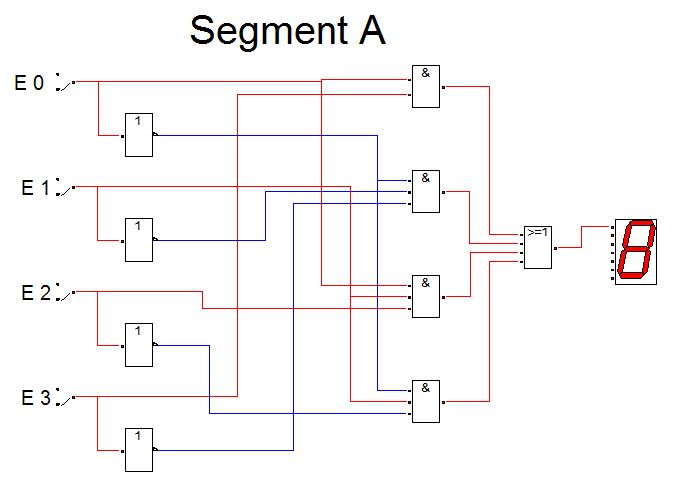
\includegraphics[width=0.75\columnwidth]{DT4Graphics/Segment_A.jpg}
\captionof{figure}{Schaltung Segment A}
\vspace{10mm}
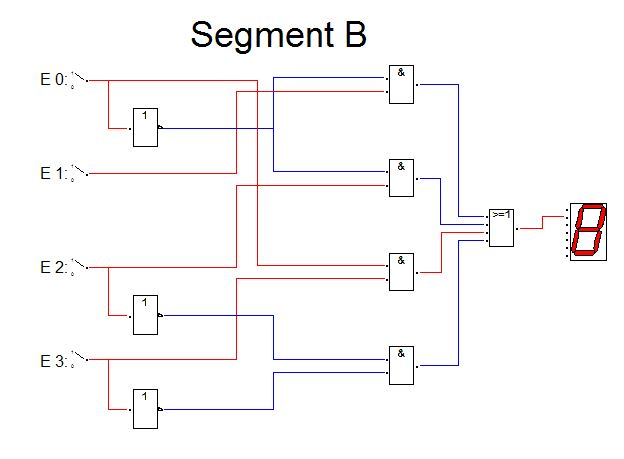
\includegraphics[width=0.75\columnwidth]{DT4Graphics/Segment_B.jpg}
\captionof{figure}{Schaltung Segment B}
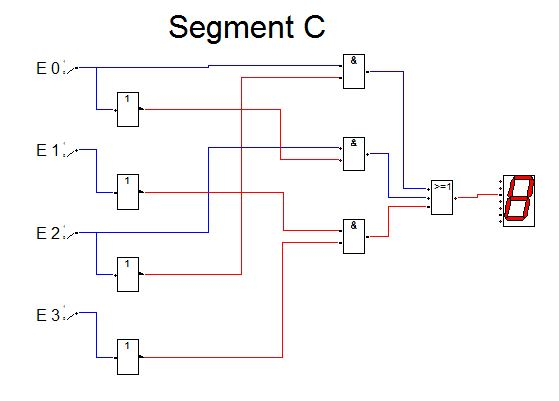
\includegraphics[width=0.75\columnwidth]{DT4Graphics/Segment_C.jpg}
\captionof{figure}{Schaltung Segment C}
\vspace{10mm}
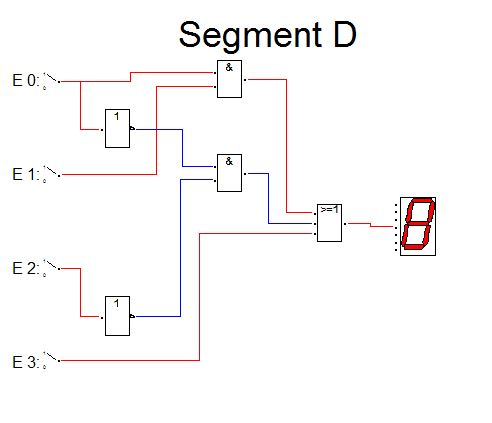
\includegraphics[width=0.75\columnwidth]{DT4Graphics/Segment_D.jpg}
\captionof{figure}{Schaltung Segment D}
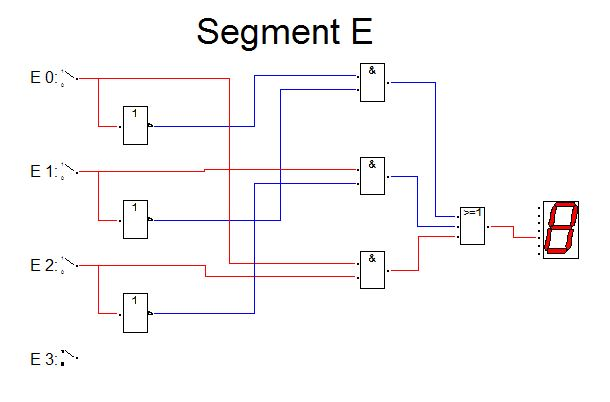
\includegraphics[width=0.8\columnwidth]{DT4Graphics/Segment_E.jpg}
\captionof{figure}{Schaltung Segment E}
\vspace{10mm}
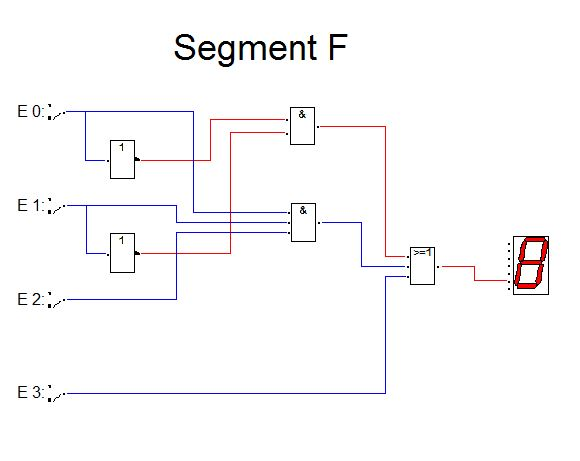
\includegraphics[width=0.75\columnwidth]{DT4Graphics/Segment_F.jpg}
\captionof{figure}{Schaltung Segment F}
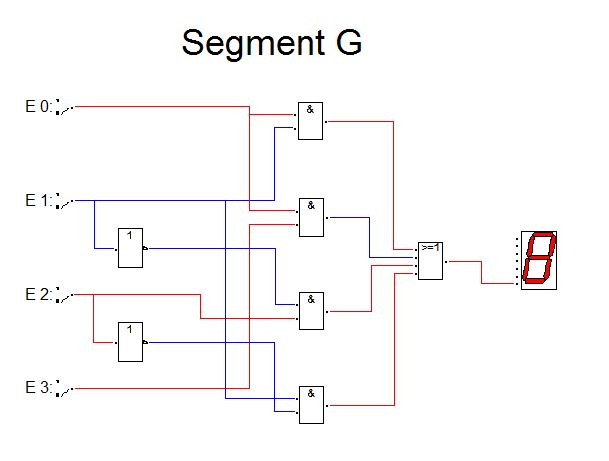
\includegraphics[width=0.8\columnwidth]{DT4Graphics/Segment_G.jpg}
\captionof{figure}{Schaltung Segment G}


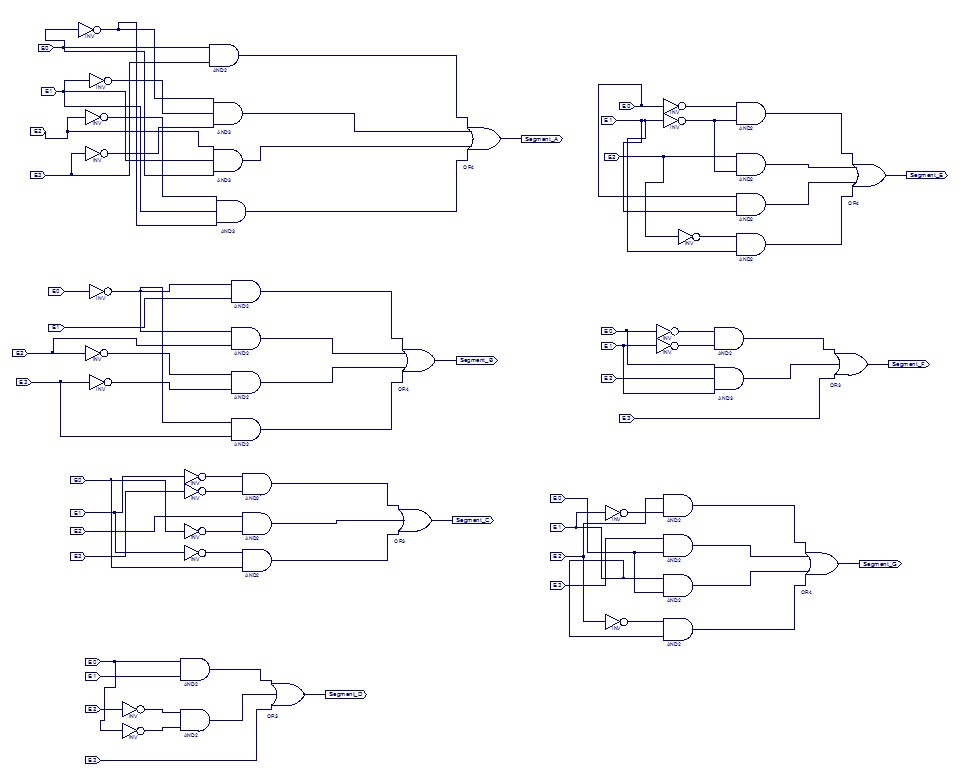
\includegraphics[width=1.2\columnwidth]{DT4Graphics/alle_schaltungen.jpg}
\captionof{figure}{Screenshot der Schaltungen vom Versuchstag}
\end{center}
\newpage
\chapter{Kritische Schlussbetrachtung}
\section{Olbrich, Marie}
 In Versuch DT4 sollte ein BCD -> 7-Segment-Kodeumsetzer entworfen und mit Hilfe eines CPLD Bausteines realisiert werden.\par 
Jede Gruppe hat einen speziellen Kode, der umzusetzen ist. Dazu sollten in den vorbereitenden Aufgaben eine Wahrheitstabelle des Kodeumsetzers und KV-Diagramme für die einzelnen Segmente erstellt werden. Aus den KV-Diagrammen wurden die speziellen Gleichungen für jedes Segment abgelesen. \par
Am Versuchstag sollte mit einem Computerprogramm die Ansteuerlogik mittels UND, ODER und NICHT Gattern entworfen werden. Es wurde für jedes Segment eine eigene Schaltung entworfen. Anschließend musste die Pin-Belegung des CPLD Bausteins festgelegt werden. Obwohl die vorbereitenden Aufgaben korrekt gelöst waren, traten zwei Fehler auf. Diese sind entstanden, weil bei zwei Segmenten Verbindungen fehlten. Diese Fehler waren jedoch schnell zu beheben und nach erneutem Kompilieren funktionierte alles einwandfrei. \par
Die vorbereitenden Aufgaben konnten ohne Probleme in der vorgegebenen Zeit gelöst werden. Während dem Versuch war die Zeit jedoch sehr knapp, da man sich zunächst in das Programm einarbeiten musste. Außerdem führte ein kleiner Schreibfehler in den Unterlagen zunächst zu Verwirrung, da ein CLPD Baustein im Internet nicht zu finden war, sondern nur ein CPLD Baustein. Deshalb herrschte kurz Unklarheit darüber, ob es sich um denselben Baustein handelt, was jedoch zu Beginn des Praktikums geklärt werden konnte und zu keinen weiteren Problemen führte.
 
\section{Hoffmann, Manuel}
Versuchsdiskussion Digitaltechnik Praktikum SS'17

Versuch DT4

In dem Versuch DT4 geht es darum, mittels eines CLPD-Bausteins, eine Sieben-Segment-Anzeige zu programmieren.
Die für jede Gruppe spezifische Code-Tabelle befindet sich in den Versuchsunterlagen. 

Zuerst sind aus der Code-Tabelle eine Wahrheitstabelle für die einzelnen Segmente A-G zu erstellen.
Anschließend sind einzelne KV-Diagramme und die dazugehörigen Schaltungsgleichungen zu erarbeiten.

Am Versuchstag selbst werden, anhand der vorbereiteten KV-Diagramme, in einem speziell dafür vorgesehenem Programm die Schaltzeichnungen der einzelnen Segmente erstellt. Im weiteren Verlauf muss man die, in den Schaltzeichnungen festgelegten, Ein- sowie Ausgänge zu den dazugehörigen Pins des CLPD-Bausteins zuweisen.

Sofern alle Arbeitsschritte wie z.B. Speichern und Kompilieren korrekt ausgeführt wurden und die Schaltzeichnungen korrekt sind funktioniert die Sieben-Segment-Anzeige wie in der Code-Tabelle vorgesehen.

Mögliche Fehlerquellen sind wie im vorliegendem Fall geschehen beispielsweise nicht korrekt verbundene Leitungen in den Zeichnungen oder auch vom Programm nicht ordnungsgemäß übernommene Pinbelegung.

%%%%%%%%%%%%%%%%%%%%%%%%%%%%%%%%%%%%%%%%%%%%%%%%%%%%%%%%%%%%%%%%%%%%%%%%%%%%%%%%%%%%%%%
%%%%%%%%%%%%%%%%%%%%%%%%%%%%%%%%%%%%%%%%%%%%%%%%%%%%%%%%%%%%%%%%%%%%%%%%%%%%%%%%%%%%%%%
%%%%%%%%%%%%%%%%%%%%%%%%%%%%%%%%%%%%%%%%%%%%%%%%%%%%%%%%%%%%%%%%%%%%%%%%%%%%%%%%%%%%%%%
%%%%%%%%%%%%%%%%%%%%%%%%%%%%% Hier fängt der Text an %%%%%%%%%%%%%%%%%%%%%%%%%%%%%%%%%%
%%%%%%%%%%%%%%%%%%%%%%%%%%%%%%%%%%%%%%%%%%%%%%%%%%%%%%%%%%%%%%%%%%%%%%%%%%%%%%%%%%%%%%%
%%%%%%%%%%%%%%%%%%%%%%%%%%%%%%%%%%%%%%%%%%%%%%%%%%%%%%%%%%%%%%%%%%%%%%%%%%%%%%%%%%%%%%%
%%%%%%%%%%%%%%%%%%%%%%%%%%%%%%%%%%%%%%%%%%%%%%%%%%%%%%%%%%%%%%%%%%%%%%%%%%%%%%%%%%%%%%%
\end{document}